\documentclass[11pt,twocolumn]{ctexart}
\usepackage[top=1in,bottom=1in,left=1in,right=1in]{geometry}
\usepackage[bf,small,pagestyles]{titlesec}
\usepackage[dvips]{graphicx}
\usepackage{float}
\usepackage{indentfirst}
\usepackage[ps2pdf=true,colorlinks]{hyperref}
\usepackage[figure,table]{hypcap} % Correct a problem with hyperref
\hypersetup{
   bookmarksnumbered,
   pdfstartview={FitH},
   citecolor={black},
   linkcolor={black},
   urlcolor={black},
   pdfpagemode={UseOutlines}
}
\usepackage{multicol}
\def\pgfsysdriver{pgfsys-dvipdfmx.def}
\pagestyle{plain}

\begin{document}
\title{\textbf{基于深度学习的X光图像违禁品检测算法}\\[1ex]YOLO 系列算法研究进展}
\author{季潇剑 2024010010}
\date{\today}

\twocolumn[
\begin{@twocolumnfalse}
\phantomsection
\addcontentsline{toc}{section}{Title}
\maketitle

\phantomsection
\addcontentsline{toc}{section}{Abstract}
\begin{abstract}
随着深度学习技术的发展,X光图像检测在公共安全领域中扮演着越来越重要的角色。YOLO(You Only Look Once)系列算法以其卓越的实时性和准确性,在目标检测领域取得了显著成就。本综述旨在全面分析YOLO系列算法在X光图像检测中的应用、进展和挑战,探讨其在公共安全领域中的潜力和未来发展方向。 
\end{abstract}
\end{@twocolumnfalse}
]
%\begin{multicols}{2}
\section{引言}
阿巴巴巴巴爸爸巴巴爸爸巴巴爸爸巴巴爸爸啊爸爸巴巴爸爸吧

\section{研究背景}


\subsection{X光图像}
X射线成像是一种高效的无损检测技术,在行李安检中被广泛用于检测隐藏的危险物品。其成像原理基于X射线管发射的高能电离射线穿透扫描对象,根据物体材料的密度和厚度导致射线信号的衰减。衰减的程度可以用公式 $I_x = I_0 e^{-\mu x}$ 表示,其中 $I_x$ 是穿透材料后的射线强度,$I_0$ 为初始射线强度,$\mu$ 为线性衰减系数,$x$ 为材料厚度 [XX]。材料的密度越高,衰减越显著,因此在图像中表现为强度较低的区域(如图3A所示)。这种物理特性使X射线成像在检测高密度危险物品(如金属武器和爆炸物)时尤为有效,同时也能够区分低密度有机材料(如塑料和液体)。

在安检应用中,目前市场上最常见的是二维X射线图像技术,因其设备相对低成本且能够快速生成行李内容的内部结构信息 [XX]。二维成像通过单能级或多能级X射线进行扫描,单能级成像利用固定能量的射线生成灰度图像(如图3-a),能够提供物体基本的密度信息。然而,单能级技术在复杂行李场景中可能难以清晰区分多种材料,例如金属、塑料和有机物的混合情况。为应对这一问题,现代X射线机广泛采用多能级成像技术,通过不同能量级别的X射线生成多张图像,结合查找表(Look-Up Table,LUT)方法,将不同材料的密度和有效原子序数($Z_{eff}$)转换为伪彩色图像(如图3B所示) [XX] 。在伪彩色图像中,高密度金属可能被标记为蓝色,而低密度有机材料则呈现为橙色或红色,从而显著增强了危险物品的可识别性。这种技术特别适用于检测复杂行李中的危险品,例如将枪支、刀具与普通物品区分开来,同时减少误报。

此外,多视角成像技术进一步提升了二维X射线成像的检测能力。多视角技术通过从不同角度对行李进行扫描,生成多张图像(如图4-a),从而提供更丰富的空间信息,使隐藏在复杂结构中的危险物品(如刀具、金属爆炸物等)更加突出,同时提高了对多层结构的解析能力 [XX]。尽管多视角成像需要更多的数据处理能力,但在实际安检中已被广泛使用,其与多能级技术结合,显著提高了检测效果。

\subsection{传统方法检测}
在深度学习技术尚未普及之前,传统的X光图像安检检测方法在相关研究中占据重要地位。这些方法主要涵盖图像增强、威胁图像投影(Threat Image Projection, TIP)、目标分类、目标检测和图像分割等技术领域,依托计算机视觉与传统机器学习手段,旨在提升X光图像的可读性和检测性能,为安检工作提供基础性技术支持。这些传统方法的研究成果在一定程度上为后续深度学习技术的发展奠定了理论和方法论基础。

图像增强技术是传统X光安检检测的关键环节,其主要目的是通过预处理提升图像质量,使操作者或算法更容易识别潜在威胁目标。常见的技术包括低能和高能X光图像的融合,以利用不同能量水平的射线穿透特性提升目标物体的显著性。此外,伪彩色技术被广泛应用于灰度图像的可视化处理,通过将灰度值映射到颜色空间显著增强目标的可视性[11, 27-29, 102]。这些增强方法虽然能够提高安检人员对目标物体的检测效率,但它们仍然受到算法设计复杂度和对环境变化适应能力的限制。

威胁图像投影(TIP)是一种用于生成合成数据集的重要传统技术,通过将二值威胁物体掩码投影到无威胁的X光图像上生成包含威胁目标的合成图像。TIP技术的优势在于,其通过仿射变换、对数变换等操作生成了多样化的合成数据,极大地丰富了数据集的规模和多样性。这不仅可以用来训练机器学习模型,还在培训人类筛查人员的过程中得到了有效应用[32-34, 103, 104]。然而,需要指出的是,TIP生成的合成图像可能在纹理细节和真实威胁物体分布方面与实际情况存在偏差,这种限制可能会对模型在实际应用中的泛化性能造成一定影响。

在目标分类任务中,传统方法主要依赖于视觉词袋(Bag of Visual Words, BoVW)模型,该方法通过特征提取与聚类构建视觉词典,再利用支持向量机(SVM)或随机森林(RF)等分类器对目标物体进行分类[38, 105-107]。此外,稀疏表示技术通过稀疏编码的方式提取图像中的高维特征,其分类性能在部分研究中表现出优势[15, 38-39, 42-43]。例如,在GDXray数据集上的研究显示,基于稀疏表示和k-NN分类器的传统方法能够取得与深度学习模型相近的性能(94.7%对比96.3%)[49]。然而,这些方法的计算复杂度较高,且对大规模、多样化数据集的适应能力有限,难以在实际安检场景中取代深度学习方法。

在目标检测方面,传统方法同样以BoVW框架为主导,并结合稀疏强度域图像描述符(SPIN)等特征提取技术,利用SVM分类器实现了较高的检测精度[18, 40, 57, 109]。此外,多视角图像的引入显著增强了检测的鲁棒性,特别是在物体发生旋转或部分遮挡的情况下,多视角数据能够提供更多的形态和纹理信息,从而提升检测性能[17, 18, 110-111]。然而,这些方法在复杂场景中往往需要依赖大量的先验知识或人工设计特征,这在一定程度上限制了其应用的广泛性和自动化程度。

传统图像分割技术最初主要依赖于固定阈值法以分离目标与背景,这种方法虽然计算简单但对噪声和光照变化的敏感性较高。随后,基于图论的分割方法逐渐兴起,如模糊相似距离、谱聚类和变分分割技术等[61, 114, 115],在小型数据集上的表现较为优异。然而,这些方法在应对复杂结构的目标分割以及大规模数据处理时,计算效率和鲁棒性方面仍存在不足。因此,它们难以直接应用于实际安检场景,特别是在要求实时性的任务中表现较为乏力。

总体而言,传统X光图像安检检测方法通过一系列图像处理与机器学习技术,为X光图像的解读和威胁物体检测提供了重要的理论支持与实践经验。这些方法不仅在提高检测精度方面发挥了积极作用,还为后续深度学习技术的发展奠定了基础。然而,这些传统方法在应对复杂场景、多样化数据以及大规模处理任务时存在明显的局限性,包括特征提取的自动化程度不足、泛化性能有限和对高效计算的依赖性较高。随着深度学习技术的快速发展,研究逐渐向更加智能化和高效的解决方案转变。这种转变不仅在检测精度和效率上带来了显著提升,同时也为X光图像安检检测领域开辟了新的研究方向与应用场景。

\subsection{深度学习方法检测}
随着深度学习技术的迅猛发展,其在X光图像安检检测中的应用研究不断涌现,与传统方法相比,深度学习方法展现出显著的性能优势与应用潜力。在早期的工作中,Jaccard等人[23]首次将卷积神经网络(CNN)应用于X光图像分类任务,并利用迁移学习技术验证了其在数据有限场景下的有效性。在枪支与非枪支的二分类任务中,即使在网络所有权重层冻结的情况下,CNN依然显著优于基于视觉词袋(BoVW)方法的支持向量机(SVM)和随机森林(RF)。更进一步的实验则表明,CNN在多类别分类问题中同样具有较高的应用前景,尤其是在类别间具有较高相似性的情况下。

在基于深度学习的目标检测任务中,多阶段方法逐渐成为研究热点。以[64]为例,其通过滑动窗口将UCL TIP数据集的X光图像分割成小块,分别提取多种特征(如强度特征、oBIF特征、PHOW特征以及CNN特征),并使用不同分类器(如SVM、RF和CNN)进行检测,结果显示基于VGG-18提取特征的RF分类器取得了最高性能(FPR:0.22\%)。同时,[65]通过比较不同输入类型对CNN性能的影响发现,双通道输入(包含原始图像及其对数变换图像)训练的VGG-19模型在分类任务中优于单通道输入模型(AUC:97\%,FPR:6\%)。

针对深度学习在X光图像生成中的应用,Zhao等人[69]提出了一种结合GAN的三阶段算法,用于扩展标注数据集的多样性和规模。该方法首先通过前景物体的角度信息对图像进行初步分类,随后利用GAN生成高质量的X光图像,并结合对抗训练策略进一步提升生成样本的质量。后续研究[101]在此基础上改进了GAN的训练机制,生成的图像在视觉质量上显著优于之前的方法。这种基于生成模型的策略不仅在小数据集场景中提高了模型的泛化能力,同时也为后续的检测任务提供了更加丰富的训练数据。

为了解决X光图像安检检测任务中常见的类别不平衡问题,Miao等人[71]提出了一个基于跨层特征融合的模型(CHR),通过将连续层的特征进行连接和冗余信息去除,优化模型对复杂背景和少见类别的检测性能。使用SIXray数据集训练ResNet-101模型时,提出的方法实现了mAP提升2.13\%的显著改进。类似研究[96]则进一步通过引入即插即用模块,利用边缘和材料信息强化注意力机制,从而显著提升了模型对检测目标的定位能力。

在跨数据集泛化能力的研究中,Caldwell等人[67]探索了深度学习模型在不同扫描仪产生的数据间的迁移性能。实验表明,由于扫描仪参数的未知性以及数据集分布差异,深度学习模型在未见数据上的表现仍具有较大挑战。进一步研究[82]则通过在DBF3和SIXray数据集上训练和验证模型,定量分析了CNN模型的泛化能力,揭示了领域转移对检测性能的显著影响。

多视图X光图像的使用也在近年来成为提升检测性能的重要方向。研究[100]通过结合多视角检测结果,验证了多视图输入在提高模型精度上的效果(R-FCN与ResNet-101结合时,多视图mAP为0.938,而单视图仅为0.798)。此外,[79]改进了Faster RCNN的结构,通过多视图池化层提取三维特征,并生成三维候选区域以进行后续检测,实验结果表明多视图方法较单视图有显著性能提升(mAP:95.56\% vs. 91.23\%)。

综上所述,基于深度学习的X光图像安检检测方法在分类、检测及生成数据扩展等多个方向均取得了显著的研究进展。然而,尽管方法种类繁多,YOLO算法凭借其端到端设计和出色的实时性,已经在安检检测任务中脱颖而出,成为该领域的重要研究方向。后续章节将重点讨论YOLO在X光图像安检检测中的相关研究及其应用前景。


\section{YOLO系列模型在X光图像检测中的应用}
光路径的定义是用于连接客户的光通路,即光通道源节点与目的节点之间的通路。一条光路径可以使用该通路的一个或几个波长。

路由是控制面的一种功能,用于选择路径和建立连接,此连接往往穿越一个或几个传送网。

在光域中,将路由过程称为RWA问题,为了选择合适的光路径来满足流量工程要求,就必须找到光路径中物理节点和链路(路由子问题),同时找到该光路径链路上的一个或几个波长(波长分配子问题),才能优化网络资源。

\subsection{YOLO 目标检测模型各版本的发展历程}

自 2016 年 YOLO(You Only Look Once)目标检测算法问世以来,该系列算法在不到十年的时间内经历了快速的迭代与演进。尤其是在应对复杂背景、小目标检测等挑战性场景方面,其表现取得了显著提升。这些技术进步使得 YOLO 系列算法逐渐成为 X 光图像违禁品检测这一关键领域的重要技术工具,为安全检查的效率与精准度提供了强有力的技术支撑。

在该系列众多版本中,YOLOv1 至 YOLOv8,以及 YOLOX 等代表性模型,以卓越的实时性能、高检测精度和轻量化设计脱颖而出,在 X 光图像违禁品检测领域得到了广泛应用。图 XX 概述了 YOLO 系列模型从 YOLOv1 到 YOLOv8 的发展历程及各版本之间的技术继承关系。本节首先将系统性地介绍 YOLOv1 至 YOLOv8 及 YOLOX 的关键改进方向与核心技术特点,以清晰勾勒出 YOLO 系列算法在目标检测领域的技术演化脉络。随后,将进一步探讨这些版本在 X 光图像检测中的具体应用实践与表现。
\subsubsection{YOLOv1}
YOLO(You Only Look Once) 是由 Redmon 等人于 2016 年提出的一种一阶段目标检测算法,它在目标检测领域具有重要的里程碑意义。与传统的两阶段检测模型(如 R-CNN 系列)相比,YOLO 基于端到端的回归策略,直接预测目标边界框的位置和类别概率,从而实现了目标检测任务的统一建模和高效处理。这种创新设计显著简化了检测流程并提升了运行速度。

YOLOv1 首次提出了将输入图像划分为 $S \times S$ 的网格的设计思路。每个网格单元负责预测 $B$ 个边界框及其置信度分数,并输出 $C$ 个类别的概率分布。具体而言,每个边界框的预测由 5 个参数组成:$(P_c, b_x, b_y, b_w, b_h)$,其中,$P_c$ 表示边界框的置信度分数,即目标是否存在及边界框预测的准确程度;$b_x$ 和 $b_y$ 是边界框中心点相对于网格单元的偏移量;$b_w$ 和 $b_h$ 分别表示边界框的宽度和高度。最终,YOLO 的输出可以被表示为一个维度为 $S \times S \times (B \times 5 + C)$ 的张量。

如图 XX 所示,YOLOv1 的骨干网络基于 GoogLeNet 的设计思路,包含 24 个卷积层和 2 个全连接层,并引入了 $1 \times 1$ 卷积以减少计算复杂度和参数量。该模型首先在 ImageNet 数据集上进行预训练,以获取通用的特征表示;随后在 PASCAL VOC 数据集上进行微调与验证。在 PASCAL VOC 2007 数据集上,YOLOv1 实现了 63.4\% 的平均精度(AP),展现出在检测速度上的显著优势。

然而,YOLOv1 的设计也存在一定的局限性。由于采用固定网格划分以及每个网格单元固定数量的边界框,模型在检测密集目标和小目标时性能受限,容易出现漏检和定位不准确的问题。此外,为了减少边界框冗余,YOLOv1 引入了非极大值抑制(Non-Maximum Suppression, NMS),用于筛选与真实框最接近且置信度最高的预测边界框。

YOLOv1 的提出开创了实时目标检测的先河,其端到端设计和统一的处理流程显著简化了目标检测过程,同时在速度和效率上取得了革命性进展。这一创新奠定了后续 YOLO 系列模型发展的坚实基础,为目标检测领域的研究和应用开辟了新的方向。
\subsubsection{YOLOv2}
YOLOv2 是由 Joseph Redmon 和 Ali Farhadi 于 2017 年提出的目标检测算法,它在 YOLOv1 的基础上进行了多项关键改进,实现了在保持实时检测性能的同时显著提升检测精度。在网络结构方面,YOLOv2 采用了更为轻量化且高效的骨干网络 Darknet-19,该网络包含 19 个卷积层和 5 个最大池化层,并通过 $1 \times 1$ 卷积层有效减少了参数量,同时增强了特征提取能力。此外,YOLOv2 使用步幅为 2 的卷积层替代部分池化层,从而在降低特征图空间分辨率的同时保留了更多的细节信息,缓解了池化操作中常见的低层次细节丢失问题。

相比 YOLOv1,YOLOv2 的改进可以归纳为以下几个核心方面,这些改进共同推动了模型性能的显著提升。首先,YOLOv2 引入了锚框机制(Anchors),通过预定义一组固定高宽比的锚框(Anchors),模型在训练过程中学习锚框与真实框之间的偏移量,从而直接预测边界框的位置、尺寸和类别分布。锚框机制显著提升了模型在检测密集目标和小目标时的表现,同时提高了边界框预测的精度。其次,YOLOv2 在每一层网络中加入了批量归一化(Batch Normalization),这不仅加速了模型的收敛速度,还显著降低了过拟合风险,提升了模型的鲁棒性。第三,YOLOv2 采用了多尺度训练(Multi-scale Training)策略,在训练过程中动态调整输入图像的分辨率(范围为 $320 \times 320$ 至 $608 \times 608$,每 10 个 epoch 随机更改一次尺寸),从而使模型能够学习不同分辨率下的特征,增强了对目标尺度变化的适应能力。

为了进一步提高模型对小目标的检测性能,YOLOv2 引入了多项优化机制。其一,通过特征融合(Passthrough 层),即后续版本中被称为特征金字塔网络(FPN)的早期形式,YOLOv2 将浅层高分辨率特征与深层语义特征通过通道拼接的方式融合,生成的特征图包含更多细节信息,从而提高了模型对小目标的检测能力。其二,YOLOv2 在训练数据中应用了K-means 聚类算法以优化锚框大小,使锚框分布更加贴合数据的实际分布特性,从而提升了模型的边界框预测质量,并减少了对无关框的学习偏差。

在性能评估上,YOLOv2 在 PASCAL VOC 2007 数据集上的平均精度(AP)达到 78.6\%,较 YOLOv1 提高了 15.2\%,并在保持实时检测速度的同时实现了显著的精度提升。此外,YOLOv2 创新性地提出了WordTree 方法,利用层级标签结构,使模型能够在 ImageNet 和 MS COCO 等大规模数据集上进行联合训练,并支持检测超过 9000 个类别的版本——即 YOLO9000。这种大规模检测能力的实现,进一步巩固了 YOLO 系列在实时目标检测领域的领先地位。
\subsubsection{YOLOv3}
YOLOv3 是由 Joseph Redmon 和 Ali Farhadi 于 2018 年提出的一种目标检测算法,通过多项改进进一步增强了模型的检测能力,同时延续了其在实时检测中的优势。YOLOv3 引入了全新的骨干网络 Darknet-53,该网络包含 53 个卷积层,并借鉴了 ResNet 的残差连接(Residual Connection)设计,从根本上缓解了深层网络中的梯度消失问题。这一设计显著提升了模型的特征提取能力,使得 YOLOv3 在 ImageNet 数据集上的分类性能与 ResNet-152 相当,但计算速度却快近两倍,充分体现了其在高效性和性能平衡上的优越性。

在目标检测任务中,YOLOv3 的改进主要体现在多尺度检测、锚框机制优化和分类方法的调整上。为提升对不同尺度目标(特别是小目标)的检测能力,YOLOv3 采用了类似于特征金字塔网络(Feature Pyramid Network, FPN)的多尺度检测机制。模型通过从不同分辨率的特征图上进行检测,分别在 13×13、26×26 和 52×52 的特征图上预测目标边界框。这种分层检测策略使得每个分辨率的特征图能够专注于特定大小目标的检测:低分辨率特征图(13×13)负责大目标的检测,中分辨率特征图(26×26)检测中等目标,而高分辨率特征图(52×52)则专注于小目标。这一设计极大地提高了模型对不同尺度目标的适应性,尤其是在复杂场景中检测小目标的能力。

在锚框机制方面,YOLOv3 延续了使用锚框(Anchors)作为边界框先验的设计,并通过 K-means 聚类对训练数据生成更合理的锚框尺寸。相比之前的版本,YOLOv3 在每种尺度的特征图上由每个网格单元预测三个边界框,这种改进进一步提升了目标尺度的建模精度。同时,在类别预测上,YOLOv3 放弃了传统的 Softmax 激活函数,转而采用独立的逻辑回归方法。这种方法不仅支持多标签分类(例如一个目标可以同时属于“动物”和“宠物”两类),还为每个边界框预测独立的类别概率,提高了分类的灵活性和对复杂场景的适应能力。此外,为了进一步提升检测性能,YOLOv3 支持引入空间金字塔池化(Spatial Pyramid Pooling, SPP)模块,通过整合不同感受野的池化特征(例如 $1\times1$、$3\times3$、$5\times5$ 和 $7\times7$),显著扩大了感受野范围,增强了模型对全局和局部特征的捕捉能力。

在 MS COCO 数据集上的评估中,YOLOv3 实现了31.0\% 的平均精度(AP)(COCO 标准),以及55.3\% 的 AP@50(即 IoU 大于 0.5 时的检测精度)。尽管在 COCO 标准下的平均精度上未能完全超越更复杂的两阶段检测器(如 Faster R-CNN 和 Mask R-CNN),但 YOLOv3 通过实现检测速度与精度的高度平衡,依然在实时检测任务中占据了重要地位,成为工程应用中的主流选择,尤其适合对实时性要求较高的场景。
\subsubsection{YOLOv4}
YOLOv4 是由 Alexey Bochkovskiy 等人于 2020 年提出的一种目标检测算法,它通过整合多种优化策略,在保持实时检测性能的同时显著提升了检测精度。YOLOv4 的架构进行了全面的设计优化,包括特征提取、特征融合和检测头三大模块。在特征提取阶段,YOLOv4 引入了 CSPDarknet-53 作为骨干网络。该网络基于 YOLOv3 的 Darknet-53 结构,结合了跨阶段部分连接(CSPNet)的设计,通过跨层连接有效减少梯度信息的冗余,提升了模型的学习效率,同时降低了计算复杂度和参数量,而不损失检测精度。此外,YOLOv4 采用了 Mish 激活函数,这是一种平滑的非线性激活函数,相较于 ReLU 和 Leaky ReLU,它在梯度流动和深层网络的稳定性上表现更为优异,从而进一步增强了特征提取能力。

在特征融合阶段,YOLOv4 结合了多项先进设计,显著提升了对不同尺度目标的检测能力。首先,通过改进版的空间金字塔池化(Spatial Pyramid Pooling, SPP)模块,模型通过多尺度池化操作(例如 $1\times1$、$5\times5$、$9\times9$ 和 $13\times13$ 的池化核),在不增加计算成本的前提下扩大了感受野范围,并增强了特征图中多尺度信息的表达能力。这种设计使得模型能够更精准地捕捉不同大小目标的轮廓特征。此外,YOLOv4 采用了路径聚合网络(Path Aggregation Network, PANet),进一步优化了特征金字塔结构中不同分辨率特征之间的信息传递,尤其是在浅层高分辨率特征与深层低分辨率特征之间的融合上表现突出,从而提升了模型对小目标检测的性能以及复杂场景下的适应性。

在模型的训练阶段,YOLOv4 集成了多种创新的优化策略,以增强训练的稳定性并提高检测性能。其中,Mosaic 数据增强是一项显著提升训练样本多样性的技术,通过随机将四张图像拼接为一张,模型在小目标检测和复杂背景适应性上表现更加出色。自对抗训练(Self-Adversarial Training, SAT)策略的引入,则通过在训练过程中生成对抗样本,使模型在面对扰动或噪声时具有更高的鲁棒性。YOLOv4 还优化了边界框回归的损失函数,使用 CIoU(Complete IoU)损失,综合考虑了边界框之间的距离、重叠度和长宽比一致性,从而显著提升了边界框定位的精度。为了减少模型的过拟合问题,YOLOv4 在训练中加入了类别标签平滑(Label Smoothing)和 DropBlock 正则化策略。前者通过对类别标签分布的平滑处理,降低了模型对训练数据的过度拟合倾向;后者则通过在特征图上随机遮挡部分区域,增强了模型的泛化能力。此外,YOLOv4 还首次在目标检测中采用了遗传算法进行超参数优化,通过自动搜索找到最佳的模型配置参数,进一步提升了性能。

在性能评估上,YOLOv4 在 MS COCO 数据集上实现了 43.5\% 的平均精度(AP),AP@50 达到 65.7\%,在精度和速度之间取得了更优的平衡。尽管在 COCO 标准下的平均精度上未能完全超越更复杂的两阶段检测器(如 Faster R-CNN 和 Mask R-CNN),但 YOLOv4 凭借其卓越的实时性和高效的性能设计,成为了工业应用中的首选模型。
\subsubsection{YOLOv5}
YOLOv5 是由 Ultralytics 公司 于 2020 年 发布的目标检测算法,与之前的 YOLO 系列相比,其在易用性 和部署性能 方面实现了显著突破。作为 YOLO 系列的延续与优化,YOLOv5 通过多项创新设计进一步提升了检测精度、运行效率和适配能力。其中,引入的 Focus 模块 、C3 模块 、SPPF 模块 和 AutoAnchor 技术 ,在不同层面优化了模型结构、锚框生成和多尺度目标的检测能力,使其成为一款更高效且易于部署的目标检测框架。

在网络结构方面,YOLOv5 通过关键模块的改进进一步增强了模型性能。首先,Focus 模块 通过对输入特征图进行切片操作实现了无损下采样,不仅大幅提高了下采样效率,还保留了更多空间细节信息,从而增强了对小目标的检测能力。其次,YOLOv5 的 C3 模块 是对 YOLOv4 中 CSP 模块 的优化,通过跨层部分连接减少梯度冗余的同时,在不显著增加参数量的前提下有效提升了特征表达能力。此外,模型还引入了 SPPF 模块(快速空间金字塔池化) ,通过整合不同尺度的特征图来增强对多尺度目标的表达能力,尤其是在复杂场景中有效捕捉多目标信息。

在锚框生成方面,YOLOv5 创新性地采用了 AutoAnchor 技术 ,能够根据训练数据集的特性和配置动态优化锚框大小。这种动态调整不仅简化了锚框参数设置的流程,还提升了模型对遮挡目标的检测精度和召回率。此外,YOLOv5 提供了全面的数据增强策略,包括 Mosaic 数据增强 、复制粘贴(Copy-Paste) 、MixUp 、随机仿射变换 和颜色变换 等,大幅提升了训练样本的多样性和模型的泛化能力,使其在复杂场景下表现更加鲁棒。

YOLOv5 的显著特点之一是模型版本的多样性 。它提供了五种不同规模的版本,分别为 YOLOv5n(纳米) 、YOLOv5s(小型) 、YOLOv5m(中型) 、YOLOv5l(大型) 和 YOLOv5x(超大型) ,以适应不同计算资源和应用需求。轻量化版本(如 YOLOv5n 和 YOLOv5s)因其极低的计算需求,非常适合部署在边缘设备或移动端环境中,而高性能版本(如 YOLOv5x)则在检测精度上表现突出。与 YOLOv4 相比,YOLOv5 显示出显著的训练速度优势,同时通过解决网格敏感性问题,提高了梯度稳定性,进一步增强了模型的训练效率和推理性能。

在性能评估中,YOLOv5 展现了卓越的检测能力和运行速度。在 MS COCO 数据集测试-dev 2017 上,YOLOv5x 在输入分辨率为 640×640 的设置下实现了 50.7\% 的平均精度(AP),在更高分辨率(1536×1536 )和测试时间增强(TTA)条件下,AP 进一步提升至 55.8\% ,充分展现了其高精度目标检测的能力。不仅如此,YOLOv5 不再局限于目标检测任务,还扩展支持了图像分类 和实例分割 任务。同时,YOLOv5 适配了移动端平台,提供了适用于 iOS 和 Android 的版本,显著提升了其跨平台部署能力和实际应用价值。这种灵活性使 YOLOv5 成为了工业应用中极具吸引力的选择,广泛应用于安防、自动驾驶和智能设备等实时检测场景,进一步巩固了其在目标检测领域的主流地位。
\subsubsection{YOLOX}
YOLOX(You Only Look Once Extended) 是由 旷视科技 于 2021 年 发布的一种目标检测模型,相较于传统的 YOLO 系列,YOLOX 在架构设计上进行了深度改进,显著提升了检测精度和训练效率,并简化了模型的实现。作为对 YOLOv3 的延续与优化,YOLOX 引入了多项创新技术,包括无锚框架(Anchor-free Design) 、解耦头(Decoupled Head) 、SimOTA 标签分配 、多正样本策略 以及高级数据增强技术 ,实现了在检测速度与精度之间的优异平衡,奠定了其在目标检测领域的重要地位。

YOLOX 的核心改进体现在以下几个方面,首先,无锚框架设计 摒弃了从 YOLOv2 起使用的锚框机制,直接预测目标的网格偏移、宽度和高度,从而简化了模型的结构和训练流程。这种无锚方案受到无锚目标检测器(如 FCOS)的启发,避免了锚框匹配过程中的超参数干扰,同时提升了模型的效率和检测性能。在 MS COCO 数据集上的实验表明,无锚框架设计使 YOLOX 的平均精度(AP)提高了 0.9 个百分点 ,并降低了训练复杂度。

此外,YOLOX 采用了解耦头(Decoupled Head)的检测结构,将分类任务和边界框回归任务分离为两个独立的子网络。这一改进解决了任务耦合带来的特征共享冲突问题,使模型在收敛速度和检测性能上均有所提升。与传统的检测头设计相比,解耦头设计进一步提高了模型的平均精度,使 AP 增加了 1.1 个百分点 。同时,YOLOX 提出了基于最优传输理论(Optimal Transport, OT)的标签分配策略 SimOTA ,从全局视角优化了正负样本的分配规则。该策略不仅有效缓解了样本不平衡和标签分配的歧义性,还显著提升了目标特征与样本匹配的质量,使 AP 增加了 2.3 个百分点 。

在无锚框架下,YOLOX 进一步引入了多正样本策略 ,通过中心采样机制,将每个预测网格的中心区域标记为正样本,从而缓解了正负样本数量的不平衡问题。这一策略显著提升了模型的检测能力,使 AP 增加了 2.1 个百分点 。同时,YOLOX 在训练阶段结合了多种高级数据增强技术 ,包括 Mosaic 数据增强 和 MixUp ,大幅扩展了训练样本的多样性。这些技术使得模型即使在没有 ImageNet 预训练的情况下,也能够取得优异的性能,并通过提升泛化能力使 AP 增加了 2.4 个百分点 ,进一步巩固了 YOLOX 在目标检测任务中的优势。

在性能评估中,YOLOX-L 在 MS COCO 测试-dev 2017 数据集上实现了 50.1\% 的平均精度(AP),表现出了卓越的检测能力。与传统锚框机制的模型相比,YOLOX 在复杂场景和大规模数据集中的表现尤为突出,同时在训练效率和模型精度方面实现了显著突破。这种高效的无锚设计和创新的优化策略,使 YOLOX 成为新一代目标检测模型的典范,在学术研究与工业应用中均展现了强大的潜力。
\subsubsection{YOLOv6}
YOLOv6 是由 美团视觉 AI 部门 于 2022 年 发布的一款目标检测模型,旨在平衡检测精度与速度,同时满足工业应用中对高效部署的需求。作为 YOLO 系列的最新发展之一,YOLOv6 在继承经典设计理念的基础上,结合多项前沿技术,对模型架构、训练策略和推理效率进行了全面优化,展现出卓越的性能和广泛的适应性。

在网络架构设计上,YOLOv6 引入了基于 RepVGG 的高效模块 EfficientRep ,通过灵活的模块设计针对不同规模的模型进行了优化。小型模型采用了 RepBlock ,而大型模型则引入 CSPStackRep 模块,显著增强了特征提取能力并提升了计算的并行性。在颈部结构上,YOLOv6 使用增强型路径聚合网络(Enhanced PAN),结合 RepBlock 构建了 RepPAN 模块,从而进一步提升了特征融合效率,使模型在处理复杂场景时表现尤为出色。同时,YOLOv6 的检测头设计为高效解耦头(Efficient Decoupled Head) ,通过分类任务与边界框回归任务的分离有效缓解了两者之间的特征冲突问题。此外,混合通道策略的引入进一步减少了计算量与推理延迟,为实现实时检测提供了可靠的技术支撑。

YOLOv6 在模型设计中摒弃了传统的锚框机制,转而采用无锚框架,通过直接预测边界框参数简化了模型结构并提升了训练效率。这一无锚设计结合了任务对齐学习(Task-Aligned One-Stage Object Detection, TOOD)策略,动态优化标签分配,以生成更多高质量的正样本,提高了检测精度。在损失函数方面,YOLOv6 使用 VariFocal Loss 优化分类任务,并通过 SIoU/GIoU 损失函数进一步提升了边界框回归的准确性。

在模型压缩与加速方面,YOLOv6 进行了系统性的优化。通过引入 RepOptimizer 和结合通道蒸馏的量化方法,模型在推理速度与精度之间实现了良好的平衡。同时,自蒸馏策略进一步降低了推理成本,使得模型的部署效率显著提升。为适应多样化的硬件资源和应用需求,YOLOv6 提供了多个版本,从轻量化的 YOLOv6-N(纳米) 到高性能的 YOLOv6-L6(超大型) ,涵盖了从边缘设备到高性能服务器的各种场景需求。

在性能表现上,YOLOv6 在 MS COCO 测试-dev 2017 数据集上展现了卓越的效果。其中,YOLOv6-L 在 NVIDIA Tesla T4 GPU 上通过 TensorRT 加速实现了 52.5\% 的平均精度(AP)和 70.0\% 的 AP@50,同时推理速度达到 29 FPS 。而更高性能的 YOLOv6-L6 模型在相同环境下取得了 57.2\% 的平均精度(AP),进一步验证了其在高精度任务中的优越性。这些结果充分证明了 YOLOv6 在速度与精度上的高度平衡,为工业应用中的实时检测任务提供了可靠的解决方案。

凭借高效的架构设计和灵活的版本选择,YOLOv6 在工业场景中展现了广泛的应用潜力。它不仅在物流分拣、视频监控等领域得到大规模应用,还为高效目标检测提供了新的思路和发展方向。其创新设计不仅推动了目标检测领域的技术进步,也为后续研究与实践奠定了坚实的理论与技术基础。
\subsubsection{YOLOv7}
YOLOv7 是由 YOLOv4 和 YOLOR 的研究团队 于 2022 年 7 月 提出的一种高效目标检测模型,其核心目标是实现检测精度与推理效率的高度平衡。与 YOLOv4 类似,YOLOv7 支持在 MS COCO 数据集 上从头开始训练,无需预训练的骨干网络。这一设计不仅简化了模型的训练流程,还显著增强了其在处理多样化数据分布时的适应能力,进一步拓展了模型的实用性。

YOLOv7 的核心架构引入了扩展高效层聚合网络(Extended Efficient Layer Aggregation Network, E-ELAN) ,这一模块在原有 ELAN 模块的基础上进行了重要改进。通过优化最短和最长梯度路径,E-ELAN 显著提升了深层特征的学习能力,同时加速了模型的收敛过程。其设计通过扩展、洗牌和合并基数等操作,在保持原始梯度路径完整性的同时有效整合了不同组间的特征,从而进一步增强了网络的表达能力。此外,YOLOv7 针对深度模型中输入与输出通道比例变化可能对硬件效率产生的影响,提出了一种基于连接的复合缩放策略。该策略在调整网络宽度和深度时,能够保持网络结构的特性,从而优化了模型的硬件推理性能,为实际应用中的部署提供了可靠支持。

为了进一步提升训练效率和检测精度,YOLOv7 在训练过程中引入了多个免费工具包(Bag-of-Freebies) ,显著优化了模型性能。首先,受 YOLOv6 中重参数化卷积(RepConv)思想的启发,YOLOv7 提出了改进版的重参数化卷积 RepConvN ,通过移除恒等连接避免了残差连接和密集连接的破坏,从而增强了卷积操作的适配性。其次,YOLOv7 在训练阶段引入了辅助检测头,采用粗略的标签分配机制为主检测头提供辅助学习信号,这种策略有效提升了训练精度,同时不影响模型的推理速度。此外,YOLOv7 采用了批量归一化重新参数化策略 ,将推理阶段的批量均值和方差整合至卷积层权重中,从而显著提升了推理效率。训练过程中,YOLOv7 还结合了隐式知识增强模型的表示能力,并通过指数移动平均(EMA)技术进一步优化了模型的推理效果和检测精度。

在性能评估中,YOLOv7 在 MS COCO 测试-dev 2017 数据集上展现了卓越的效果。在输入图像大小为 640×640 的条件下,YOLOv7 实现了 51.4\% 的平均精度(AP)和 69.7\% 的 AP@50,充分体现了其强大的检测能力和高效的设计理念。凭借其高效性与可靠性,YOLOv7 在目标检测领域取得了显著的技术突破。其创新的模型设计和卓越的性能表现,使其成为实际应用中的理想选择,为实时目标检测任务提供了更加优越的解决方案。
\subsubsection{YOLOv8}
YOLOv8 是由 Ultralytics 团队 于 2023 年 1 月 发布的最新目标检测模型。在继承 YOLO 系列优秀特性的基础上,YOLOv8 通过多项改进显著提升了检测精度和灵活性,同时保持了高效的推理速度。其主干网络基于 CSPDarknet-53 ,并将传统的 C3 模块 替换为具有更多残差连接的 C2f 模块 (一种跨阶段部分瓶颈模块)。这一设计优化了梯度流和特征提取能力,在几乎不增加计算成本的情况下,显著提高了模型对小目标和复杂场景的适应能力。此外,YOLOv8 延续使用了 SPPF(快速空间金字塔池化) 模块,通过整合多尺度信息,进一步增强了特征表达能力。

在检测头部分,YOLOv8 采用了解耦头(Decoupled Head)结构,将分类任务与边界框定位任务分离,允许两者独立优化,从而显著提升了检测精度。与此同时,YOLOv8 摒弃了传统的锚框机制,转而采用无锚点设计(Anchor-free Design) ,从根本上简化了训练与推理流程,同时减少了参数量与计算复杂度。在损失函数方面,YOLOv8 引入了分布焦点损失(DFL)和 CIoU 损失 ,并结合任务对齐分配器优化了正负样本分配策略。这些改进显著增强了目标分类和边界框预测的性能,使模型在精度和效率上达到了更高的平衡。

在训练策略方面,YOLOv8 同样进行了优化。例如,尽管马赛克数据增强在训练早期能够显著提高模型性能,但在训练后期可能对精度产生负面影响。针对这一问题,YOLOv8 采用了动态增强策略,在训练的最后 10 个 epoch 阶段关闭马赛克增强,从而提升了模型在实际应用中的稳定性和精度。此外,为满足不同应用场景和计算资源的需求,YOLOv8 提供了五种规模的模型:N(纳米) 、S(小型) 、M(中型) 、L(大型) 和 X(超大型) ,从轻量化版本到高性能版本均有覆盖,能够灵活适配多样化的应用场景。

值得一提的是,YOLOv8 扩展支持了语义分割任务,其语义分割版本 YOLOv8-Seg 在检测头后集成了分割模块,用于预测输入图像的分割掩码。在实际评估中,YOLOv8-Seg 在语义分割与目标检测任务中均表现出卓越的性能。例如,在 MS COCO 测试-dev 2017 数据集上,YOLOv8X 在输入尺寸为 640×640 像素的条件下达到了 53.9\% 的平均精度(AP) 。

凭借其卓越的性能、灵活的设计以及高效的部署能力,YOLOv8 成为目标检测和语义分割领域中不可忽视的重要工具。其多样化的模型规模和广泛的任务适配性,使其不仅适用于学术研究,也在工业应用中展现了巨大的潜力,为实时检测和分割任务提供了新的解决方案。



\subsection{评价指标}
\subsection{数据集介绍}
\subsection{YOLO各版本在X光图像检测中的应用}

\subsection{模版参考内容}
光网络构架的演进是从传统的不透明到全光网透明架构。图~\ref{EVO}转自\cite{1}展示了其光网络的演进.
\begin{figure}[!hbtp]
  \begin{center}
  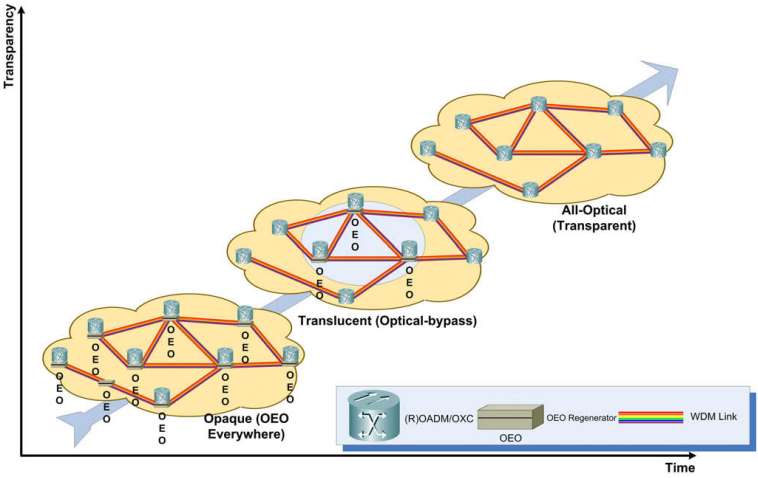
\includegraphics[width=0.5\textwidth]{EVO}
  \end{center}
  \caption{光通信网络的演进}
  \label{EVO}
\end{figure}

光信号的传输要通过在每个光交换或路由处的OEO转换。由于时机和经济的考虑,光信号的传输距离是有限的(e.g. 2000-2500km)。为了超越这个极限,信号的再生(re-amplify, re-shape and re-time, 称为3R)是至关重要的。然而在光信号的传输过程中,如果能更有效地降低其物理损伤,光信号的传输效率也能明显地提高,同时信号的再生所需的工作也能从一定程度上减轻。

物理层的损伤可以被看成是对路由和波长分配决定的一种约束 (i.e. physical layer impairment constrained (PLIC-RWA));或是有路由和波长分配来考虑之(i.e. physical layer impairment aware (PLIA-RWA))。在后者中,找到合适物理损伤的路由决定是可能的。简单地说既考虑物理损伤的路由和波长分配决定(PLI-RWA)。其算法可以简单归纳如下:

首先利用经典RWA算法从可用资源中选路,其次是计算该波长路径上的物理损伤,验证该光路上的信号至目的节点时其OSNR值(光信噪比, Optical Signal Noise Rate)能否满足最低需求,如能满足需求则使用该光路建立连接,否则换下一条光路验证其物理损伤情况。图~\ref{IRWA}转自\cite{8}显示了其算法的基本步骤.
\begin{figure}[!hbtp]
  \begin{center}
  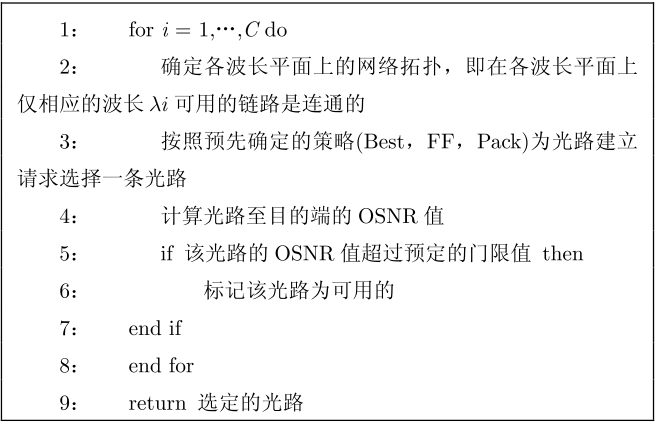
\includegraphics[width=0.5\textwidth]{IRWA}
  \end{center}
  \caption{具有损伤感知能力的动态RWA算法}
  \label{IRWA}
\end{figure}


光层组播是指通过在物理层对组播数据进行复制, 并使用光分波器/合波器等无源器件实现点到多点的连接。在WDM网络中实现光层组播首先要建立点到多点的光连接方式, 从而形成光组播树, 并为其分配波长, 即RWA。周迎富等人利用分层图模型提出光组播树多路径波长优化算法。图~\ref{MT}转自\cite{8}显示了其模型.
\begin{figure}[!hbtp]
  \begin{center}
  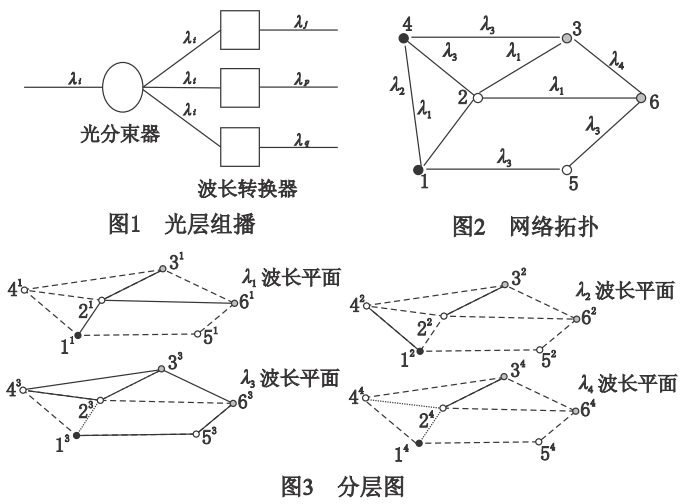
\includegraphics[width=0.5\textwidth]{MT}
  \end{center}
  \caption{基于网络编码的光组播树优化RWA模型}
  \label{MT}
\end{figure}


Goran Z. and Teodorovic D 等人提出了基于蜜蜂群优化算法(Bee Colony Optimization, BCO)的RWA(BCO-RWA)。\cite{6} BCO-RWA算法从某种程度上看是一种路由拓扑结构,通过对这种拓扑结构的阐释和理解,对光传输的路由进行选择,从而优化RWA的问题。

模型通过模拟蜜蜂群选择路线来确定路由的最佳路线,其模拟的网络由即RWA。周迎富等人利用分层图模型提出光组播树多路径波长优化算法。图~\ref{BCO}转自\cite{6}显示。
\begin{figure}[!hbtp]
  \begin{center}
  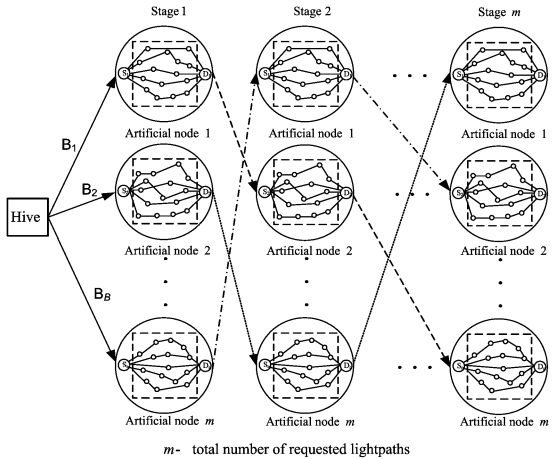
\includegraphics[width=0.5\textwidth]{BCO}
  \end{center}
  \caption{基于蜜蜂群算法的虚拟网络}
  \label{BCO}
\end{figure}


通过对第三章中几种典型的优化RWA算法,比较无线传感器中的一些路由协议,我觉得对于在光通信中的RWA虽然是一个NP问题,但其实质上是一个优化路由问题。其目的并不是要完全的解决它,而是尽一切可能的去优化,使之能够达到应用层面的需求。

对于第一种IRWA,可以对比到无线传感器中的能量认知路由(Energy-aware routing)。在无线传感器网络中,能源的约束是决定网络生命期的最主要因素。因此对于节点间的通信,以及节点与基站的通信都应该以尽可能减少能量开销为考虑的首要因素。针对此点,很多人也建立了各种各样的模型来达到此目的。比如,在通信前选好路径、将不活动的节点处于休眠状态、设置数据门限(当数据变化量大于某值才发送信号)等一系列的模型使各种不同的路由方式能适应各种不同的网络需要。我认为IRWA也能借鉴这些模型中的一部分来完成光通信网络的需要。

对于第二种基于网络编码的光组播树优化RWA模型,无线传感器网络中也有对应的路由模型。等级路由(hierarchical routing)就是一种典型的基于簇状的路由方式。其模型将网络节点分为各个等级,最简单的是挑出一部分作为一簇节点中的“簇头”,这样,数据线从各节点传出,先经过簇头的封装优化,再传送给基站;同样,如果基站需要的数据在哪一个簇,它可以直接和簇头联系,而避免了广播需求而消耗的大量能量。图~\ref{TEEN}转自\cite{11}显示了一种典型的无线传感器网络等级路由协议。
\begin{figure}[!hbtp]
  \begin{center}
  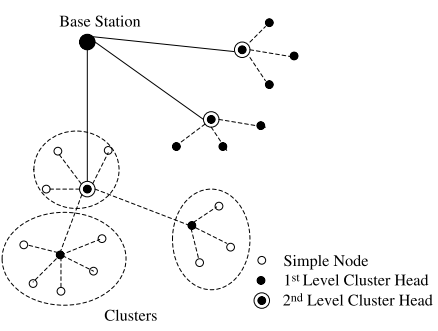
\includegraphics[width=0.5\textwidth]{TEEN}
  \end{center}
  \caption{TEEN和APTEEN中的等级簇}
  \label{TEEN}
\end{figure}

而对于基于蜜蜂群优化算法的RWA,是一种比较特殊的优化算法,Goran Z.等人在将这种算法运用到RWA问题上时做了大量的计算仿真以及比较\cite{6}。正如文中所说,这种算法具有一定的可行性,并且其性能也很优秀于很多其他模型,但是由于其复杂程度以及不确定性等因素,只能适用于相应需求的光网络系统。

事实上,由于光网络通信中有各种各样的需求与条件,不论是哪一种模型,都是基于某种或某些条件而建立的,并不能完全的适合各种网络需求。这样我们只能尽可能的利用不同的模型方式来满足各种不同的网络需求。



\phantomsection 
\addcontentsline{toc}{section}{References}
\begin{thebibliography}{99}
\bibitem{1} Siamak Azodolmolky et al.,
	{\it A survey on physical layer impairments aware routing and wavelength assignment algorithms in optical networks}
	Computer Networks, Dec. 2008
	
\bibitem{2} Hamza Drid, Bernard Cousin, Miklos Molnar, Samer Lahoud,
	{\it A Survey of Survivability in Multi-Domain Optical Networks}
	Computer Communications, 2010 
	
\bibitem{3} Huan Song, Byoung-Whi Kim, and Biswanath Mukherjee 
	{\it Long-Reach Optical Access Networks: A Survey of Research Challenges, Demonstrations, and Bandwidth Assignment Mechanisms}
	 IEEE Communications Survey and Tutorials, accepted, 2009

\bibitem{4} Huan Song et al.,
	{\it Long-Reach Passive Optical Networks}
	cs.ucdavis.edu, 2009
	
\bibitem{5} Ravinder Yadav, Rinkle Rani Aggarwal,
	{\it Survey and Comparison of Optical Switch Fabrication Techniques and Architectures}
	Department of Computer Science and Engineering, Thapar University, Patiala, 2010
	
\bibitem{6} G.Z., Teodorovic~D., Acimovic-Raspopovic V.S.,
	{\it Routing and Wavelength Assignment in All-Optical Networks Based on the Bee Colony Optimization}
	AI Communications - The European Journal on Artificial Intelligence, (in press).
	 
\bibitem{7} Martin Maier, Martin Reisslein,
	{\it Trends in Optical Switching Techniques: A Short Survey}
	IEEE Network, 2008

\bibitem{8} 赵继军, 王丽荣, 纪越峰, 徐大雄,
	{\it 基于损伤感知的动态RWA算法性能比较研究}
	电子与信息学报, Mar. 2010

\bibitem{9} 周迎富, 阳小龙,
	{\it 基于网络编码的光组播树优化RWA研究}
	计算机应用研究, Nov. 2009

\bibitem{10} 李景聪, 吴德明, 徐安士
	{\it IP over WDM光网络及其生存性问题讨论}
	光电子$\cdot$激光 Feb. 2002
	
\bibitem{11} Kemal Akkaya, Mohamed Younis 
	{\it A survey on routing protocols for wireless sensor networks}
	Nov.~2003
	
\end{thebibliography}
%\end{multicols}
\end{document}
